\chapter{Configuration}

Les étapes de configuration de MySQL et icCube converge vers l'objectif commun d'avoir un cube OLAP sur lequel il est possible d'effectuer des requètes multi-dimensionnelles. 

\section{Importation des données dans MySQL}

Après avor créé un nouvel utilisateur MySQL, nous avons importé les données du dump \texttt{aventure2014.sql.gz}.

Les données importées proviennent d'une base de données fournie par Microsoft. Il s'agit de 120'000 ventes d'articles de vélo, par internet et en magasin dans plusieurs pays. Le diagramme ER\footnote{Entity-Relationship} est visible sur la figure \autoref{img:er-diagramm}. 

\begin{figure}[H]
    \centering
    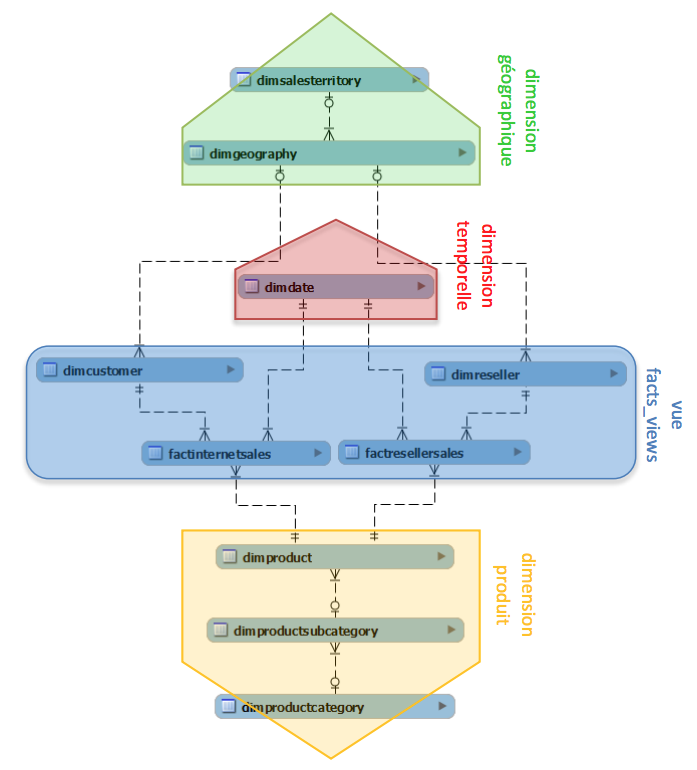
\includegraphics[width=0.7\linewidth, fbox]{img/er_diagramm.png}
    \caption{Entity Relationship diagramm}
    \label{img:er-diagramm}
\end{figure}

\subsection{Création d'une vue}

Pour préparer les différentes dimensions que nous souhaitons avoir avec notre cube OLAP, une vue supplémentaire est nécessaire. Il s'agit de la \texttt{product\_view} qui a été créée avec la requète \autoref{lst:sqlProductView}

\begin{figure}[H]
\centering
\begin{lstlisting}	
CREATE VIEW product_views AS 
SELECT dp.ProductKey, dp.EnglishProductName, dp.ProductSubcategoryKey, dps.EnglishProductSubcategoryName, dps.ProductCategoryKey, dpc.EnglishProductCategoryName 
FROM dimproduct AS dp 
LEFT JOIN dimproductsubcategory AS dps 
ON dps.ProductSubcategoryKey = dp.ProductSubcategoryKey 
LEFT JOIN dimproductcategory AS dpc 
ON dpc.ProductCategoryKey = dps.ProductCategoryKey
\end{lstlisting}
\caption{Requête SQL pour la création de la vue des produits}
\label{lst:sqlProductView}
\end{figure}


\section{Configuration d'icCube}

\subsection{Dimension temporelle}

% Pour la dimension temporelle, vous créerez 2 hiérarchies (Année → Mois → Jour / Année → Semestre → Trimestre → Jour). 
%Vous mettrez, dans votre rapport, des captures d’écran des différents paramètres.

\subsubsection*{Hiérarchie Année - Mois - Jour}

\begin{figure}[H]
    \centering
    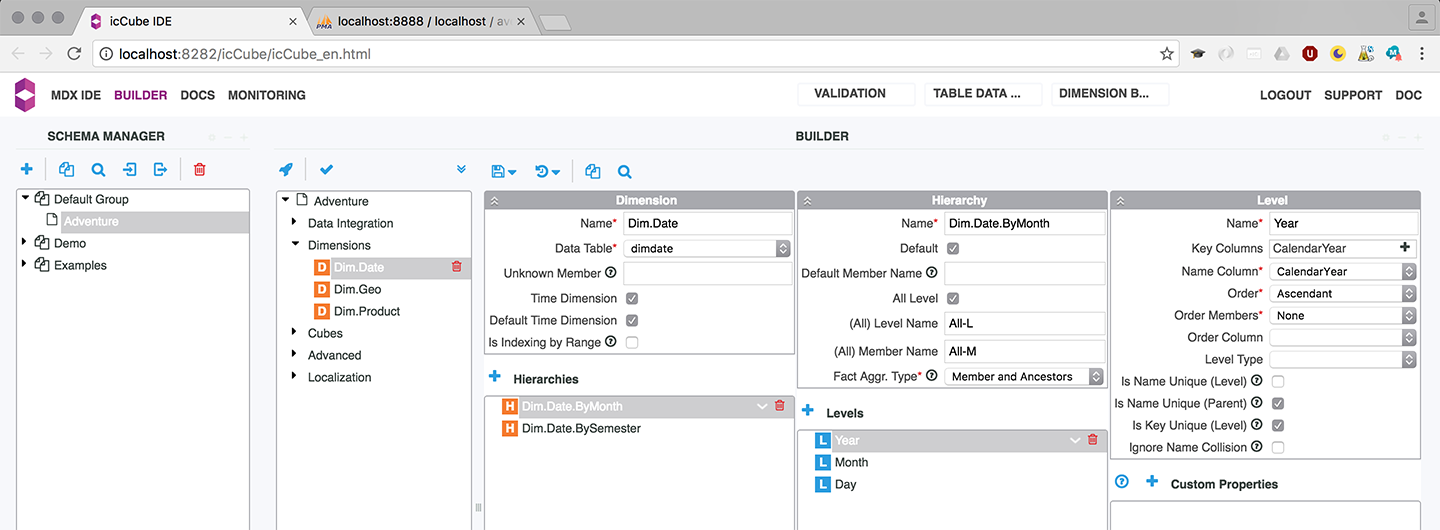
\includegraphics[width=1\linewidth, fbox]{img/dateMonthYear.png}
    \caption{Configuration Dim.Date.ByMonth - Year}
    \label{dateMonthYear}
\end{figure}

\begin{figure}[H]
    \centering
    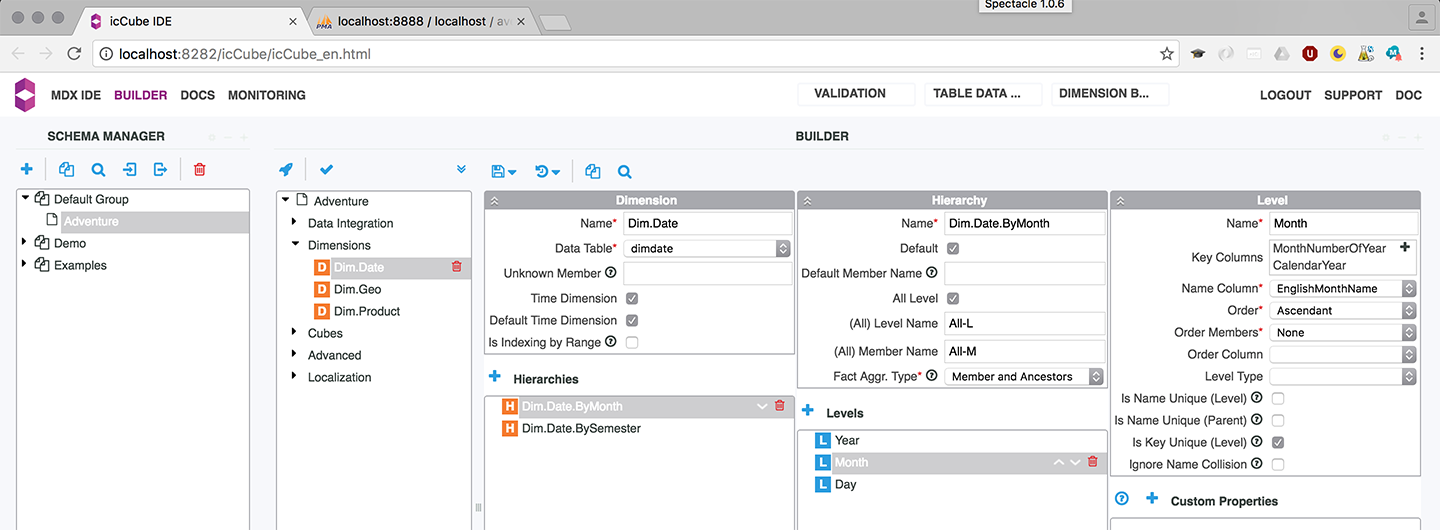
\includegraphics[width=1\linewidth, fbox]{img/dateMonthMonth.png}
    \caption{Configuration Dim.Date.ByMonth - Month}
    \label{dateMonthMonth}
\end{figure}

\begin{figure}[H]
    \centering
    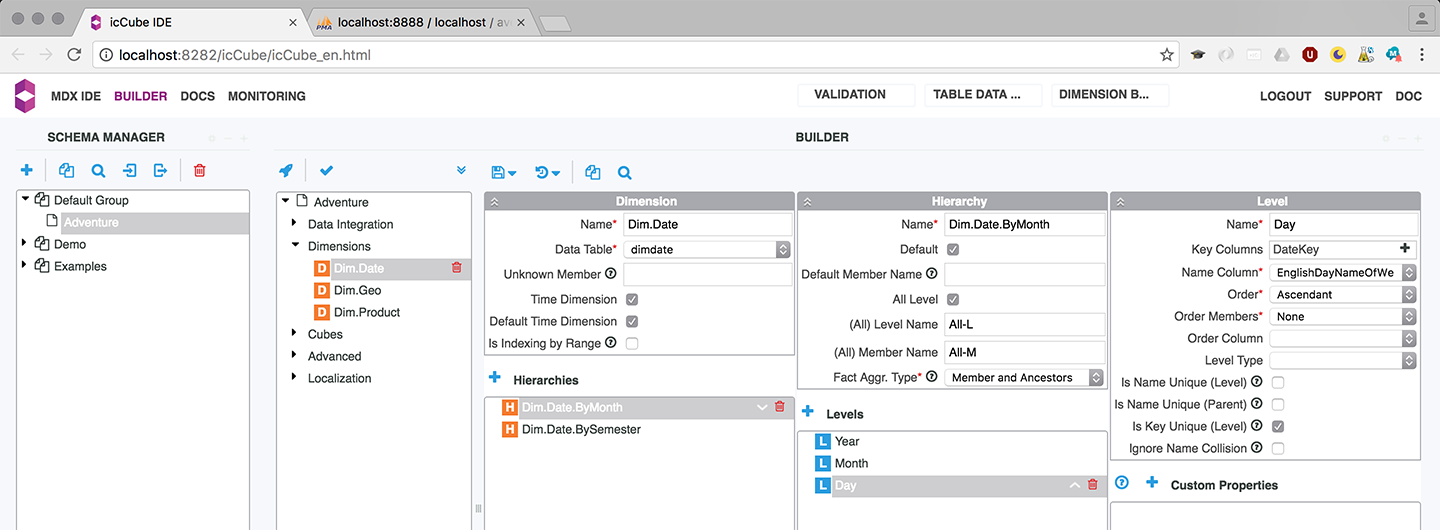
\includegraphics[width=1\linewidth, fbox]{img/dateMonthDay.png}
    \caption{Configuration Dim.Date.ByMonth - Day}
    \label{dateMonthDay}
\end{figure}

\subsubsection*{Hiérarchie Année - Semestre - Trimestre - Jour}

\begin{figure}[H]
    \centering
    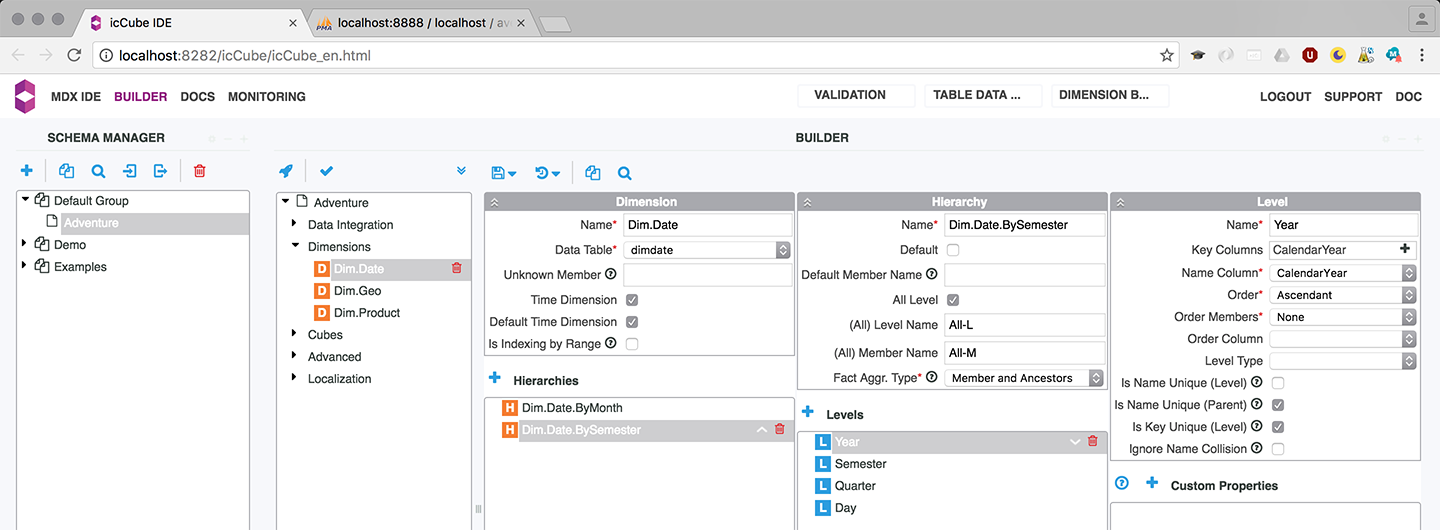
\includegraphics[width=1\linewidth, fbox]{img/dateSemYear.png}
    \caption{Configuration Dim.Date.BySemester - Year}
    \label{dateSemYear}
\end{figure}

\begin{figure}[H]
    \centering
    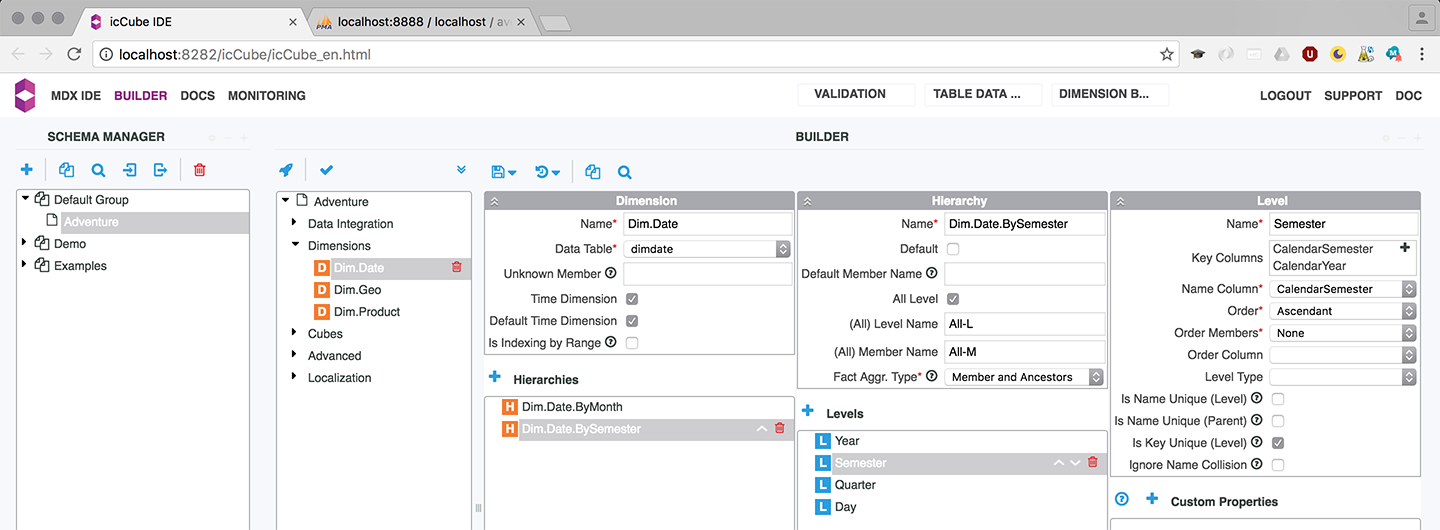
\includegraphics[width=1\linewidth, fbox]{img/dateSemSem.png}
    \caption{Configuration Dim.Date.BySemester - Semester}
    \label{dateSemSem}
\end{figure}

\begin{figure}[H]
    \centering
    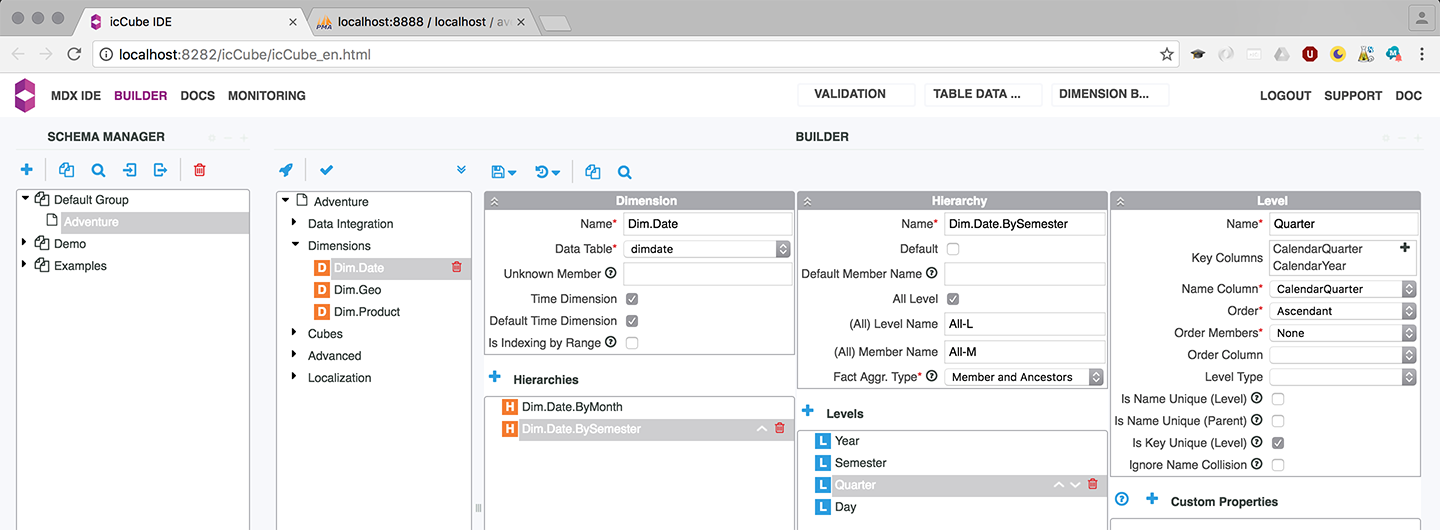
\includegraphics[width=1\linewidth, fbox]{img/dateSemQuarter.png}
    \caption{Configuration Dim.Date.BySemester - Quarter}
    \label{dateSemQuarter}
\end{figure}

\begin{figure}[H]
    \centering
    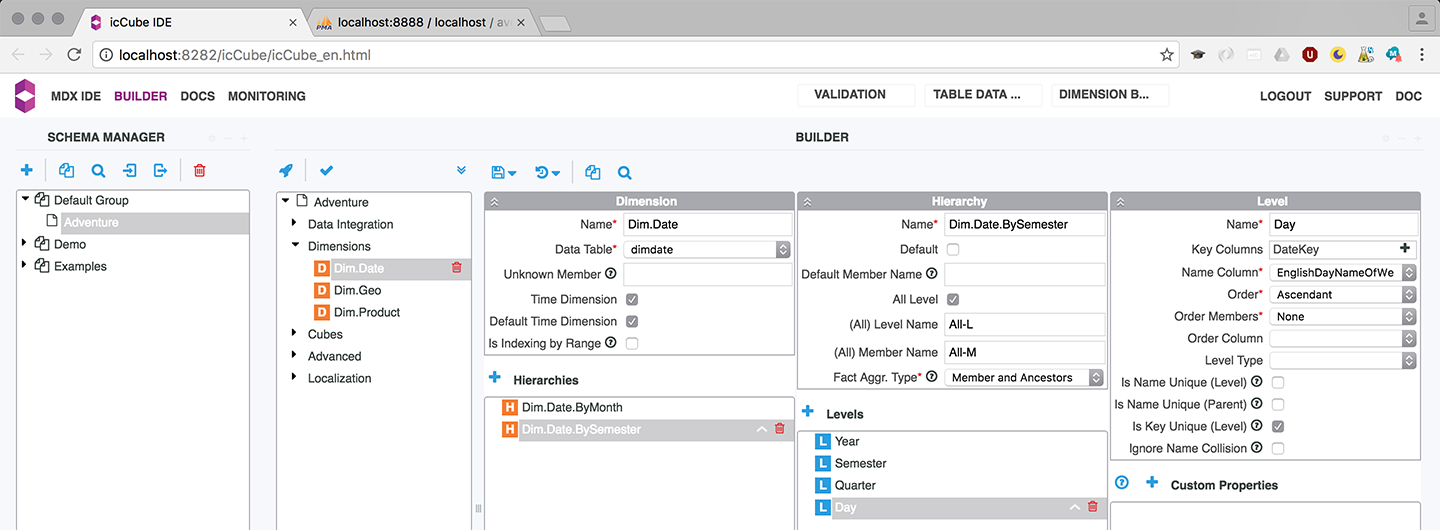
\includegraphics[width=1\linewidth, fbox]{img/dateSemDay.png}
    \caption{Configuration Dim.Date.BySemester - Day}
    \label{dateSemDay}
\end{figure}



\subsection{Dimension des produits}

% Pour la dimension des produits, les informations nécessaires sont réparties dans différentes tables, vous devrez donc utiliser la vue MySql que vous avez créée (point 1). 
% Veuillez aussi mettre des captures d’écran dans votre rapport.

\begin{figure}[H]
    \centering
    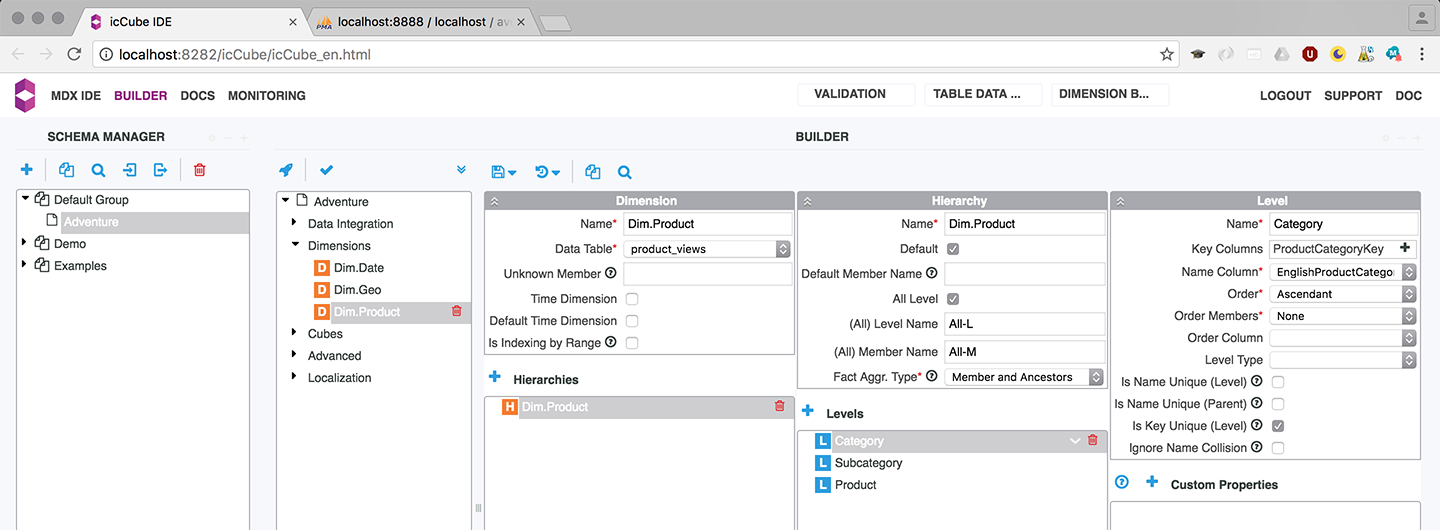
\includegraphics[width=1\linewidth, fbox]{img/prodCat.png}
    \caption{Configuration Dim.Product - Category}
    \label{prodCat}
\end{figure}

\begin{figure}[H]
    \centering
    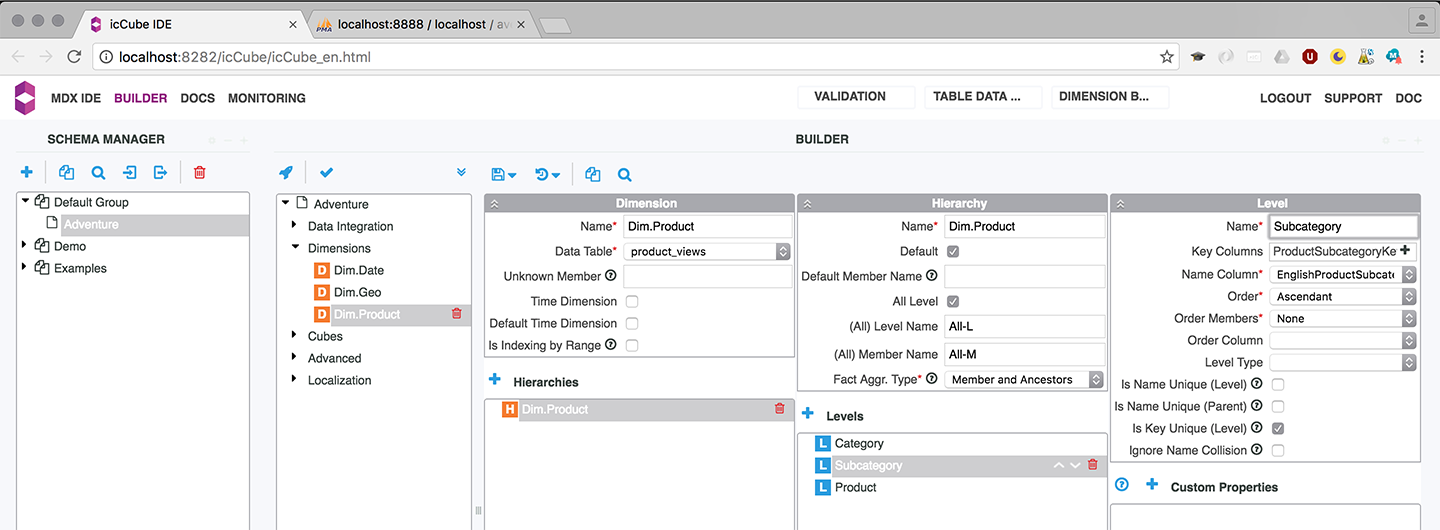
\includegraphics[width=1\linewidth, fbox]{img/prodSubcat.png}
    \caption{Configuration Dim.Product - Subcategory}
    \label{prodSubcat}
\end{figure}

\begin{figure}[H]
    \centering
    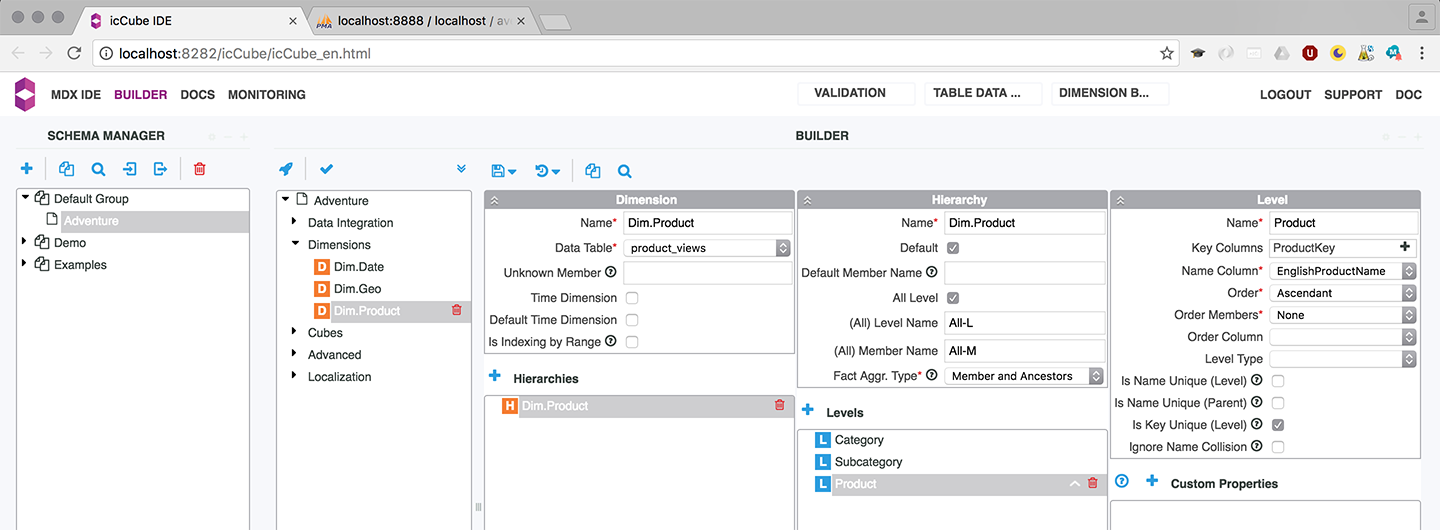
\includegraphics[width=1\linewidth, fbox]{img/prodProd.png}
    \caption{Configuration Dim.Product - Product}
    \label{prodProd}
\end{figure}





